\documentclass[a4paper,12pt]{article} \usepackage{graphicx}
\usepackage{epstopdf} %\usepackage{gensymb} \usepackage{longtable}
\usepackage{graphicx}
\usepackage{listings}
\usepackage{caption}
\usepackage{subcaption}
\usepackage{morefloats}
\lstset{
        language=verilog,
        basicstyle=\footnotesize,
        breaklines=true
}

%% Definitioner för LIPS-dokument

\usepackage[english,swedish]{babel}
\usepackage[utf8]{inputenc}
\usepackage[T1]{fontenc}
\usepackage{times}
\usepackage{ifthen}

\usepackage[margin=25mm]{geometry}

\usepackage{fancyhdr}
\pagestyle{fancy}
\lhead{}
\chead{\textbf{\LIPSprojekttitel}}
\rhead{\textbf{\textsl{LiTH}}\\\textbf{\LIPSdatum}}
\lfoot{\textbf{\LIPSkursnamn}\\\textbf{\LIPSdokumentansvarig}}
\cfoot{\textbf{\LIPSprojektgrupp}\\\textbf{\LIPSgruppepost}}
\rfoot{\textbf{\textsc{Lip}s}\\\textbf{Sida~\thepage}}

\setlength{\parindent}{0pt}
\setlength{\parskip}{1ex plus 0.5ex minus 0.2ex}


\newcommand{\twodigit}[1]{\ifthenelse{#1<10}{0}{}{#1}}
\newcommand{\dagensdatum}{\number\year-\twodigit{\number\month}-\twodigit{\number\day}}

%% ------------------------------------------
% NYBILD
% Skapar centrerad bild med caption
%   
% #1: Filens url relativt '/bilder/'
% #2:  Caption
% #3: Label
% #4: Skalning
%% ------------------------------------------
\newcommand{\nyBild}[4] 
{\begin{figure}[H]
  \centering
 \includegraphics[angle=0,scale=#4]{bilder/#1}
  \caption{#2}
  \label{fig:#3}
\end{figure}}



%%  Redefinitions of commands containing @
\makeatletter
\makeatother

\newcommand{\LIPStitelsida}{%
{\ }\vspace{45mm}
\begin{center}
  \textbf{\Huge \LIPSdokumenttyp}
\end{center}
\begin{center}
  {\Large Editor: \LIPSredaktor}
\end{center}
\begin{center}
  {\Large \textbf{Version \LIPSversion}}
\end{center}
\vfill
\begin{center}
  {\large Status}\\[1.5ex]
  \begin{tabular}{|*{3}{p{40mm}|}}
    \hline
    Reviewed & \LIPSgranskare & \LIPSgranskatdatum \\
    \hline
    Approved & \LIPSgodkannare & \LIPSgodkantdatum \\
    \hline
  \end{tabular}
\end{center}
\newpage
}


\newenvironment{LIPSprojektidentitet}{%
{\ }\vspace{45mm}
\begin{center}
  {\Large PROJECT IDENTITY}\\[0.5ex]
  {\small
  \LIPSartaltermin, \LIPSprojektgrupp\\
  Linköpings Tekniska Högskola, ISY
  }
\end{center}
\begin{center}
  {\small Group member}\\
%  \begin{tabular}{|p{30mm}|p{40mm}|p{35mm}|p{45mm}|}
  \begin{tabular}{|l|p{45mm}|p{25mm}|l|}
    \hline
    \textbf{Name} & \textbf{Responsibility} & \textbf{Phone} & \textbf{E-mail} \\
    \hline
}%
{%
    \hline
  \end{tabular}
\end{center}
\begin{center}
  {\small
    %\textbf{E-postlista för hela gruppen}: \LIPSgruppepost\\
    %\textbf{Hemsida}: \LIPSgrupphemsida\\[1ex]
    \textbf{Customer}: \LIPSkund\\
    \textbf{Customer Contact}: \LIPSkundkontakt\\
    \textbf{Course Leader}: \LIPSkursansvarig\\
    \textbf{Tutor}: \LIPShandledare\\
  }
\end{center}
\newpage
}
\newcommand{\LIPSgruppmedlem}[4]{\hline {#1} & {#2} & {#3} & {#4} \\}



\newenvironment{LIPSdokumenthistorik}{%
\begin{center}
  Document history\\[1ex]
  \begin{small}
    \begin{tabular}{|l|l|p{60mm}|l|l|}
      \hline
      \textbf{Version} & \textbf{Date} & \textbf{Changes} & \textbf{Edited by} & \textbf{Reviewed} \\
      }%
    {%
      \hline
    \end{tabular}
  \end{small}
\end{center}
}
\newcommand{\LIPSversionsinfo}[5]{\hline {#1} & {#2} & {#3} & {#4} & {#5} \\}

\newcounter{LIPSkravnummer}
\newcounter{LIPSunderkravnummer}[LIPSkravnummer]

\newenvironment{LIPSkravlista}{%
  \begin{tabular}{|p{25mm}|p{25mm}|p{85mm}|p{5mm}|}
    }%
  {%
    \hline
  \end{tabular}
}

\newenvironment{LIPSleveranslista}{%
  \begin{tabular}{|p{25mm}|p{20mm}|p{65mm}|p{25mm}|p{5mm}|}
    }%
  {%
    \hline
  \end{tabular}
}


\newcommand{\LIPSkrav}[3]
{\hline
\stepcounter{LIPSkravnummer}\textbf{Krav nr \arabic{LIPSkravnummer}} &
\textbf{{#1}} & 
{#2} & 
\textbf{{#3}} 
\\}

\newcommand{\LIPSleverans}[4]
{\hline
        \textbf{{#1}} & 
        {#2} & 
        {#3} & 
        \textbf {{#4}} 
\\}

\newcommand{\LIPSunderkrav}[3]{\hline\stepcounter{LIPSunderkravnummer}\textbf{Requirement nr \arabic{LIPSkravnummer}\Alph{LIPSunderkravnummer}} & \textbf{{#1}} & {#2} & \textbf{{#3}} \\}





%%% Local Variables: 
%%% mode: latex
%%% TeX-master: "kravspec_mall"
%%% End: 


\newcommand{\degree}{\ensuremath{^\circ}}
\newcommand{\LIPSartaltermin}{2013/VT}
\newcommand{\LIPSkursnamn}{TSEK06}
\newcommand{\LIPSprojekttitel}{DLL Based Frequency Multiplier}

\newcommand{\LIPSprojektgrupp}{Group 7}

\newcommand{\LIPSgruppepost}{}
\newcommand{\LIPSgrupphemsida}{} 
\newcommand{\LIPSdokumentansvarig}{Gustav Svensk}

\newcommand{\LIPSkund}{ISY, Linköpings universitet, 581\,83 Linköping}

\newcommand{\LIPSkundkontakt}{Amin Ojani}
\newcommand{\LIPSkursansvarig}{Atila Alvandpour}
\newcommand{\LIPShandledare}{Amin Ojani}

\newcommand{\LIPSdokumenttyp}{Layout Design} 
\newcommand{\LIPSredaktor}{Nora Björklund} 
\newcommand{\LIPSversion}{1.0} 
\newcommand{\LIPSdatum}{\dagensdatum}

\newcommand{\LIPSgranskare}{} 
\newcommand{\LIPSgranskatdatum}{}
\newcommand{\LIPSgodkannare}{} 
\newcommand{\LIPSgodkantdatum}{}

\begin{document}
\LIPStitelsida

%% Argument till \LIPSgruppmedlem: namn, roll i gruppen, telefonnummer, epost
\selectlanguage{swedish}
\begin{LIPSprojektidentitet}
 
\LIPSgruppmedlem{Nora Björklund}{Project leader}{076 7756
789}{norbj648@student.liu.se}
\LIPSgruppmedlem{\LIPSdokumentansvarig}{Documentation}{073
6208776}{grulfen3@gmail.com} 
\LIPSgruppmedlem{Christopher Hallberg}{}{0739845945}{chrha007@student.liu.se} 
\LIPSgruppmedlem{Gustaf Bengtz}{}{0707367307}{gbengtz@gmail.com} 
\LIPSgruppmedlem{Johan Berneland}{}{0704988329}{johbe915@student.liu.se}
\end{LIPSprojektidentitet}

\selectlanguage{english}

\tableofcontents{} 
\newpage %% Argument till \LIPSversionsinfo: versionsnummer, datum, Ändringar,
         %  utfört av,granskat av
\addcontentsline{toc}{section}{Document history}
\begin{LIPSdokumenthistorik} 
        \LIPSversionsinfo{0.1}{}{First draft.}{}{}
\end{LIPSdokumenthistorik} 
\newpage

\section{Time Report}
% Bifogas

\section{Project Desciption}
% Kort beskrivning med motivering och mål.
% Blocknivå beskrivning liknande från tidigare rapporter

\subsection{Phase Detector}
The Phase Detector (PD) is used check whether the 360\degree delayed
signal has got a rising edge before or after the system clock. If the
360\degree delayed clock rises before the system clock, the output
from the PD is 0, and if it rises after the system clock the output is 1.
This is used to tell the counter whether it should count up or down.
\subsection{Counter}
\subsubsection{Enable Net}
\subsubsection{Bitcell}
\subsubsection{TFF and DFF}
\subsection{Digitally Controlled Delay Line}
\subsubsection{Delay Block}
\subsection{Lock Detector}
To dampen and prevent jitter effects and to save power a lock detector
has been implemented. As described in both the high level and the
transistor level report the lock detector takes two signals and if
the delay between them are within a certain interval the output is
low, otherwise high.
\subsection{Frequency Multiplier}
\subsubsection{Transition Detector}
\subsubsection{Edge Combiner}
\subsubsection{Toggle Pulsed Latch}

\section{Simulation Result}
% Testresultat, typiska tester. Med PAD-frame och allt
\subsection{Whole System Simulation}
\subsubsection{Corner simulations}
\subsubsection{Temperature simulations}
\subsubsection{Power usage}
\subsection{Phase Detector}
The most interesting aspect of the PD is the time
needed for the PD to set-up. The set-up time is how long
 before the rising edge of the clock that the data needs 
 to arrive to be sure to be noted by the PD this clock-period.

The set-up time for the PD is as follows:

tm: 144ps

wo: 178ps

wz: 108ps

wp: 84ps

\subsection{Counter}
\subsection{Digitally Controlled Delay Line}
\subsection{Lock Detector}
The important feature of the lock detector is the delay interval where
the lock signal goes low. In the figures below, an average of the
output signal from different delays between the input clock and the
360\degree delayed clock are shown. At 0 the delay between the input
signals are 0, at -100 the 360\degree delayed clock comes 100 ps
before the reference clock and reverse at 100 ps. In figure
\ref{fig:LDtm} the interval for the typical mean can be seen. The interval 
is quite even and locks when the delay between the reference
clock and the 360\degree delayed clock is approximately 50 ps, or less. Figure \ref{fig:LDwp} to
\ref{fig:LDws} show the lock interval in the corner simulations. They are
fairly uneven and shifted to the right, if compared to the typical mean.

\begin{figure}[h]
  \centering
  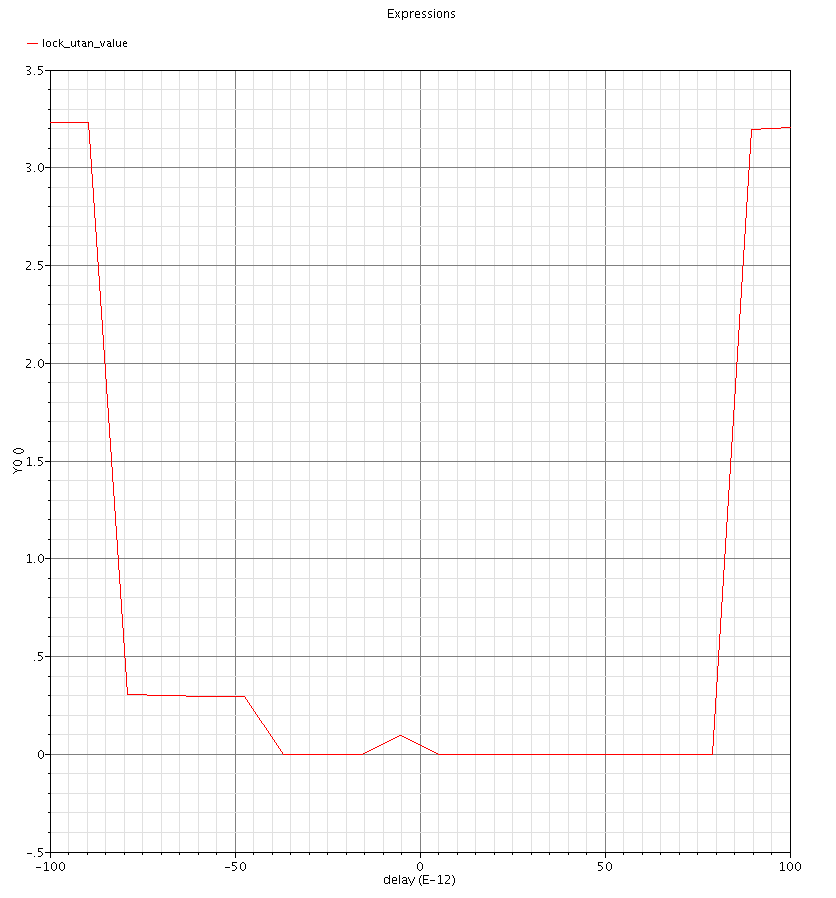
\includegraphics[width=0.65\textwidth]{../Bilder/LD_tran/LD_lsim_tm.png}
  \caption{Lock interval in typical mean}
  \label{fig:LDtm}
\end{figure}

\begin{figure}[h]
  \centering
  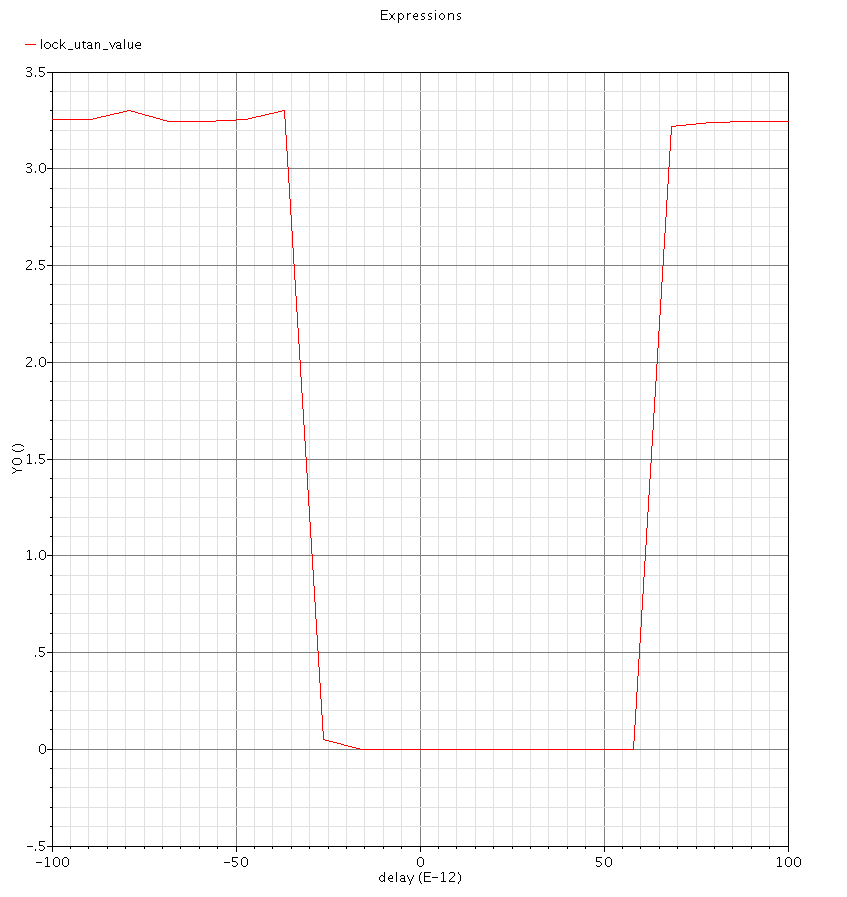
\includegraphics[width=0.65\textwidth]{../Bilder/LD_tran/LD_lsim_wp.png}
  \caption{Lock interval in worst power}
  \label{fig:LDwp}
\end{figure}

\begin{figure}[h]
  \centering
  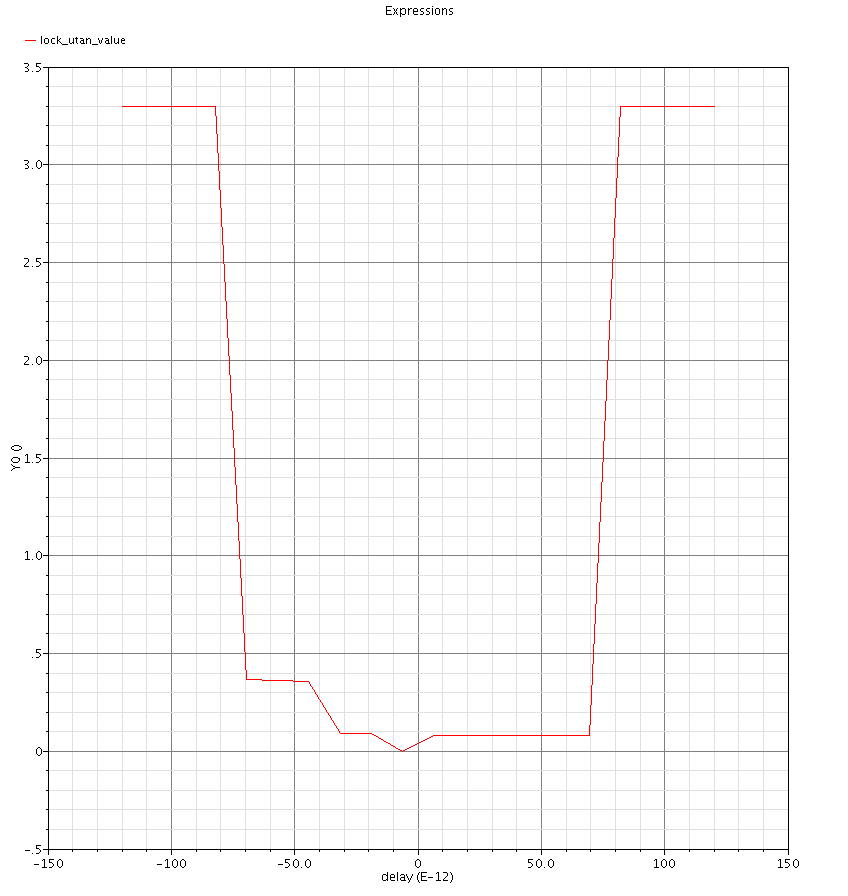
\includegraphics[width=0.65\textwidth]{../Bilder/LD_tran/LD_lsim_wo.png}
  \caption{Lock interval in worst one}
  \label{fig:LDwo}
\end{figure}

\begin{figure}[h]
  \centering
  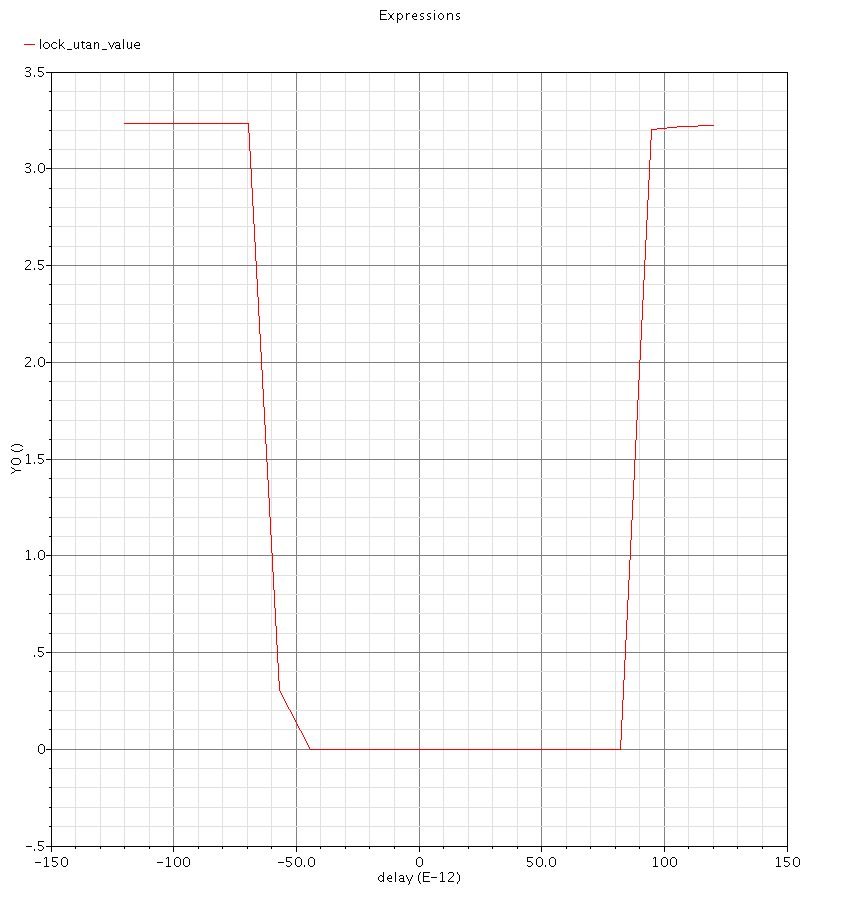
\includegraphics[width=0.65\textwidth]{../Bilder/LD_tran/LD_lsim_wz.png}
  \caption{Lock interval in worst zero}
  \label{fig:LDwz}
\end{figure}

\begin{figure}[h]
  \centering
  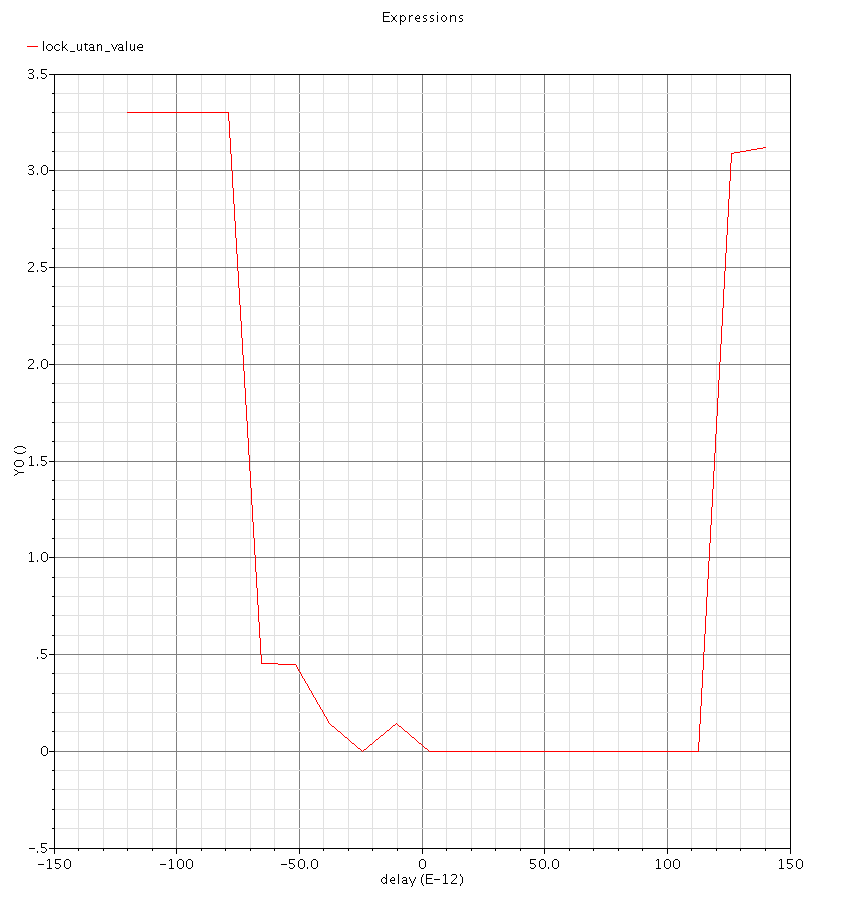
\includegraphics[width=0.65\textwidth]{../Bilder/LD_tran/LD_lsim_ws.png}
  \caption{Lock interval in worst slow}
  \label{fig:LDws}
\end{figure}

\clearpage

\subsection{Frequency Multiplier}

\section{Evaluation Plan and PAD List}
% Hur ska chippet testas?
% Vilken sorts PAD vart?
% Meningen med alla pinnar
% Sketch hur kontakterna ska kopplas till omvärlden

\section{Risks}
% Vad kan gå fel
\subsection{Phase Detector}
One of the biggest risks concerning the PD is when we get
slow/slow transistors, since the PD is used both as a stand-alone
module, and within the lock detector.
\subsection{Counter}
\subsection{Digitally Controlled Delay Line}
\subsection{Lock Detector}
\subsection{Frequency Multiplier}

\section{Evaluation}
% Vad har vi lärt oss
% Hur har gruppen fungerat
% Har tiden delats väl
% Vad var bra/dåligt
% Vad bör ändras
% Kommentarer till kursen

\newpage
\appendix 
\newpage

\addcontentsline{toc}{section}{References}
\begin{thebibliography}{99}
        \bibitem{dll_clock}\textit{A Low-Power Digital DLL-Based Clock Generator in Open-Loop Mode - }
                Behzad Mesgarzadeh, Atila Alvandpour \\
                IEEE Journal of Solid-State Circuits. Vol. 44. No. 7. July 2009
        \bibitem{lock_detect}\textit{A 62.5-625-Mhz Anti-Reset All-Digital Delay-Locked Loop - }
                Shao-Ku Kao, Bo-Jiun Chen and Shen-Iuan Liu \\
                IEEE Transations on Circuits and Systems - II: Express Briefs, Vol. 54 No. 7, July 2007
        \bibitem{dll_report}\textit{DLL-Based Frequency Multiplier - }
                Layout Edition 2008-05-25 

\end{thebibliography}
\end{document} 
% Local Variables: %%% mode: latex %%% TeX-master: t %%% End:
